<<<<<<< HEAD
% Created 2017-12-13 mié 17:46
=======
% Created 2017-12-28 Thu 22:44
>>>>>>> 2be7514637f12ec760f501e4f20932b85ca30e50
% Intended LaTeX compiler: pdflatex
\documentclass[11pt]{article}
\usepackage[utf8]{inputenc}
\usepackage[T1]{fontenc}
\usepackage{graphicx}
\usepackage{grffile}
\usepackage{longtable}
\usepackage{wrapfig}
\usepackage{rotating}
\usepackage[normalem]{ulem}
\usepackage{amsmath}
\usepackage{textcomp}
\usepackage{amssymb}
\usepackage{capt-of}
\usepackage{hyperref}
\usepackage[margin=3cm]{geometry}
\usepackage{xfrac}
\date{\today}
\title{Estructures Algebraiques: Tema 1}
\hypersetup{
 pdfauthor={},
 pdftitle={Estructures Algebraiques: Tema 1},
 pdfkeywords={},
 pdfsubject={},
 pdfcreator={Emacs 25.3.1 (Org mode 9.1.3)}, 
 pdflang={English}}
\begin{document}

\maketitle
\setcounter{tocdepth}{4}
\tableofcontents


\section{{\bfseries\sffamily TODO} Grup}
<<<<<<< HEAD
\label{sec:orgb5e1a65}
\section{{\bfseries\sffamily TODO} Interseccio, unio, producte i generacio}
\label{sec:org9a70c74}
\section{Elements d'un grup}
\label{sec:orgf1497ba}
\subsection{Definicio Centre}
\label{sec:org28ffbe0}
Sigui G un grup, llavors el Centre G es \(\mathcal{Z}(G) = \{ a \in G \mid aba^{-1} = b \quad \forall b \in G \} = \{ a \in G \mid ab = ba \quad \forall b \in G \}\).

\subsection{Definicio Centralitzador}
\label{sec:orgcf82755}
Sigui G un grup, i H un subgrup de G llavors el Centralitzador de H en G es \(\mathcal{Z}_{G}(H) = \{ a \in G \mid aba^{-1} = b \quad \forall b \in H \} = \{ a \in G \mid ab = ba \quad \forall b \in H \}\).

\subsection{Definicio Normalitzador}
\label{sec:org873eeff}
Sigui G un grup, i H un subgrup de G, llavors el normalitzador de H en G es N\(_{\text{G}}\)(H) = \(\{ a \in G \mid aHa^{-1} = H \} = \{ a \in G \mid aH = Ha \}\).

\subsubsection{Observacio:}
\label{sec:org4dc1c75}
Normalitzador de H en G = G \(\iff H \vartriangleleft G\)
\section{{\bfseries\sffamily TODO} Ordre d'un element, grup ciclic}
\label{sec:org46c3a92}
\section{{\bfseries\sffamily TODO} Morfismes de grups}
\label{sec:org1005c95}
\section{Classes laterals}
\label{sec:org1e25445}
\subsection{Definicio}
\label{sec:orgacf7c2a}
Sigui G un grup i H in subgrup de G. \(a,b \in G\). \\
Definim \(a \sim b (esquerra) \iff a^{-1}b \in H\)
\subsection{Definicio de la classe d'equivalencia}
\label{sec:org5a6b813}
=======
\label{sec:org654da55}
\section{{\bfseries\sffamily TODO} Interseccio, unio, producte i generacio}
\label{sec:orgeb1d7e2}
\section{Elements d'un grup}
\label{sec:orge2e4030}
\subsection{Definicio Centre}
\label{sec:org0ed0424}
Sigui G un grup, llavors el Centre G es \(\mathcal{Z}(G) = \{ a \in G \mid aba^{-1} = b \quad \forall b \in G \} = \{ a \in G \mid ab = ba \quad \forall b \in G \}\).

\subsection{Definicio Centralitzador}
\label{sec:org470512c}
Sigui G un grup, i H un subgrup de G llavors el Centralitzador de H en G es \(\mathcal{Z}_{G}(H) = \{ a \in G \mid aba^{-1} = b \quad \forall b \in H \} = \{ a \in G \mid ab = ba \quad \forall b \in H \}\).

\subsection{Definicio Normalitzador}
\label{sec:org4cdd146}
Sigui G un grup, i H un subgrup de G, llavors el normalitzador de H en G es N\(_{\text{G}}\)(H) = \(\{ a \in G \mid aHa^{-1} = H \} = \{ a \in G \mid aH = Ha \}\).

\subsubsection{Observacio:}
\label{sec:orgb61e528}
Normalitzador de H en G = G \(\iff H \vartriangleleft G\)
\section{{\bfseries\sffamily TODO} Ordre d'un element, grup ciclic}
\label{sec:org8fbc9a1}
\section{{\bfseries\sffamily TODO} Morfismes de grups}
\label{sec:orga1cb53e}
\section{Classes laterals}
\label{sec:orgcc06de2}
\subsection{Definicio}
\label{sec:orge22c4b2}
Sigui G un grup i H in subgrup de G. \(a,b \in G\). \\
Definim \(a \sim b (esquerra) \iff a^{-1}b \in H\)
\subsection{Definicio de la classe d'equivalencia}
\label{sec:orgdbca37a}
>>>>>>> 2be7514637f12ec760f501e4f20932b85ca30e50
\(\bar{a}\) := \{ \(b \in G\) | \(a \sim b\)\} \\
\(aH\) := \{ \(ax\) | \(x \in H\)\} \\
Observem que aH = \(\bar{a}\) \\
A més H i aH tenen el mateix cardinal.

\subsection{Definicio Classe Lateral:}
<<<<<<< HEAD
\label{sec:orgf656255}
=======
\label{sec:org4564883}
>>>>>>> 2be7514637f12ec760f501e4f20932b85ca30e50
Anomenem \(G/H = \{aH | a \in G\}\) el conjunt de les classes laterals per l'esquerra (conjunt quocient). \\
Diem també que l'índex de H en G es \([G:H] = |G/H|\) = nombre d' elements de G modul H

\subsubsection{Observacio:}
<<<<<<< HEAD
\label{sec:orgd9bfe68}
=======
\label{sec:org4d34938}
>>>>>>> 2be7514637f12ec760f501e4f20932b85ca30e50
\begin{enumerate}
\item El nombre de classes laterals per l'esquerra es el mateix que el nombre de classes laterals per la dreta.
\item L'índex és multiplicatiu. \(K \subset H \subset G\). Llavors \([G:K] = [G:H] * [H:K]\)
\end{enumerate}

\subsection{Teorema de Lagrange}
<<<<<<< HEAD
\label{sec:orgd671b39}
Sigui G un grup i H un subgrup, G finit. \\
Aleshores \(|G| = |G/H| * |H| \iff |G/H| = \frac{|G|}{|H|}\), i a més |H| divideix |G|.

\subsubsection{{\bfseries\sffamily TODO} Demo}
\label{sec:orgf59f5f9}

\section{Subgrup normal, Grup quocient}
\label{sec:org35fe8d0}
\subsection{Definicio: Subgrup Normal}
\label{sec:org3519ded}
Sigui G un grup, H un subgrup de G. H és subgrup normal de G si aH = Ha \(\forall\) a \(\in\) G.
\subsection{Lema}
\label{sec:orgc970438}
=======
\label{sec:org14f755e}
Sigui G un grup i H un subgrup, G finit. \\
Aleshores \(|G| = |G/H| * |H| \iff |G/H| = \frac{|G|}{|H|}\), i a més |H| divideix |G|.

\subsubsection{Demo}
\label{sec:org23c402c}
    Tenim G = \(\bigsqcup_{i=1}^{r} x_{i}\) Unio disjunta de classes laterals. Com \(\rvert  x_{i}H_{i}  \lvert =  \rvert  H  \lvert\) Tenim que: \\
\(\lvert G  \rvert = \sum_{i=1}^{r}  \lvert H  \rvert \iff  \lvert \sfrac{G}{H} \rvert = \frac{\lvert G \rvert}{\lvert H \rvert}\), i a mes \(\lvert H \rvert\) es divisor de  \(\lvert G \rvert\)  

\section{Subgrup normal, Grup quocient}
\label{sec:orgabb190f}
\subsection{Definicio: Subgrup Normal}
\label{sec:org1aeac77}
Sigui G un grup, H un subgrup de G. H és subgrup normal de G si aH = Ha \(\forall\) a \(\in\) G.
\subsection{Lema}
\label{sec:org70170a1}
>>>>>>> 2be7514637f12ec760f501e4f20932b85ca30e50
f: \(G_1 \to G_2\) morfime de grups. Aleshores,
\begin{enumerate}
\item Si \(H_1 \vartriangleleft G1 \implies f(H_1) \vartriangleleft f(G_1)\).
\item Si \(H_2 \vartriangleleft G2 \implies f^{-1}(H_2) \vartriangleleft G_1\).
\end{enumerate}
\subsubsection{{\bfseries\sffamily TODO} Demo}
<<<<<<< HEAD
\label{sec:org03556a0}
\subsection{Observacio}
\label{sec:org177d011}
\(H \subseteq K \subseteq G\), H,K subgrups de G. Aleshores. \\
Si \(H \vartriangleleft G \implies H \vartriangleleft K\). El reciproc es fals.
\subsection{Observacio}
\label{sec:orgf5c36e5}
si \(H \vartriangleleft G\), aleshores (aH)*(bH) = (ab)H
\subsection{Definicio: Operacio interna}
\label{sec:org6bda7f8}
=======
\label{sec:orgf6f7e65}

\subsection{Observacio}
\label{sec:orgd4f9a1e}
\(H \subseteq K \subseteq G\), H,K subgrups de G. Aleshores. \\
Si \(H \vartriangleleft G \implies H \vartriangleleft K\). El reciproc es fals.
\subsection{Observacio}
\label{sec:org4dd9b0d}
si \(H \vartriangleleft G\), aleshores (aH)*(bH) = (ab)H
\subsection{Definicio: Operacio interna}
\label{sec:org66e0d8d}
>>>>>>> 2be7514637f12ec760f501e4f20932b85ca30e50
Sigui \(H \vartriangleleft G\) i sigui G/H = \{aH | a \(\in\) G\} el conjunt de classes laterals per l'esquerra modul H. En G/H definim l'operacio interna:
\begin{alignat*}{5}
G/H &\times G/H &\to&\hspace{2pt}  G/H & \\
aH &\times bH &\mapsto&  (ab)H &
\end{alignat*}
\subsection{Corol.lari}
<<<<<<< HEAD
\label{sec:org01a65fb}
\(G/H\) es un grup i s'anomena el grup quocient de G per H.
\subsection{Exercici: La aplicacio quocient es un morfisme}
\label{sec:org6aa000f}

\section{Primer teorema d'isomorfisme}
\label{sec:orgf4556b5}

\subsection{{\bfseries\sffamily TODO} Teorema:}
\label{sec:org4f685b4}
=======
\label{sec:org77bd451}
\(G/H\) es un grup i s'anomena el grup quocient de G per H.
\subsection{Exercici: La aplicacio quocient es un morfisme}
\label{sec:org92e8893}

\section{Primer teorema d'isomorfisme}
\label{sec:org237e4eb}

\subsection{Teorema:}
\label{sec:org276f6ed}
>>>>>>> 2be7514637f12ec760f501e4f20932b85ca30e50
Sigui \(f: G_1 \to G_2\) morfisme de grups, Sigui \(H \vartriangleleft G_1\), i sigui l'aplicació

\begin{alignat*}{2}
\tilde{f}: G_1/H &\to G_2 \\
aH &\mapsto \tilde{f}(aH) := f(a)
\end{alignat*}
Aleshores\\
\begin{enumerate}
\item \(\tilde{f}\text{ ben definida }\iff H \subseteq Ker(f)\)
\end{enumerate}
Si esta ben definida:
n2. \(\tilde{f}\) es morfisme de grups
\begin{enumerate}
\item \(\tilde{f}\) injectiva \(\iff\) H = Ker(f)
\item \(Im( \tilde{f} ) = Im(f)\)
\end{enumerate}

En particular, \(\sfrac{G_1}{Ker(f)} \cong Im(f)\)
\begin{figure}[htbp]
\centering
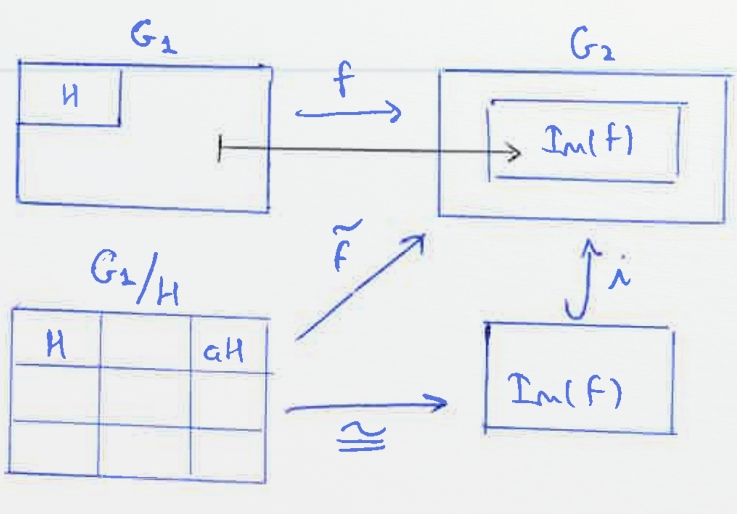
\includegraphics[width=.9\linewidth]{./images/primeriso.jpg}
<<<<<<< HEAD
\caption{\label{fig:orgd18b264}
=======
\caption{\label{fig:org2501d25}
>>>>>>> 2be7514637f12ec760f501e4f20932b85ca30e50
Primer teorema d'isomorfisme}
\end{figure}

\subsubsection{{\bfseries\sffamily TODO} demo}
\label{sec:org5cebc73}

\subsubsection{Col\(\cdot\)lorari}
\label{sec:org63e7750}
Tots els grups ciclics d'ordre n son isomorfs a \(\sfrac{\mathbb{Z}}{n\mathbb{Z}}\)

\section{El grup multiplicatiu d'un cos finit}
<<<<<<< HEAD
\label{sec:org964d2ac}

\subsection{Definicio}
\label{sec:org725ce93}
=======
\label{sec:org4707214}

\subsection{Definicio}
\label{sec:org620864a}
>>>>>>> 2be7514637f12ec760f501e4f20932b85ca30e50
Sigui \(\mathbb{K}\) un cos. El grup multiplicatiu de \(\mathbb{K}\) és \\
\begin{equation*}
\mathbb{K}^* = \mathbb{K} \setminus \{0\} = \{x \in \mathbb{K} \mid x \neq 0\}
\end{equation*}

\subsection{Teorema}
<<<<<<< HEAD
\label{sec:org36d75b9}
Sigui \(\mathbb{K}\) un cos. Sigui G un subgrup finit de \(\mathbb{K}^*\). Aleshores G és cíclic

\subsubsection{{\bfseries\sffamily TODO} demo}
\label{sec:org5059f11}

\section{Grup simples}
\label{sec:org6302674}
\subsection{Definicio}
\label{sec:orgba15b2f}
Sigui G un grup no trivial. Direm que G es simple si els unics subgrups normals de G son \{1\} i G.
\subsection{Proposicio}
\label{sec:org3f658bb}
=======
\label{sec:org104c809}
Sigui \(\mathbb{K}\) un cos. Sigui G un subgrup finit de \(\mathbb{K}^*\). Aleshores G és cíclic

\subsubsection{{\bfseries\sffamily TODO} demo}
\label{sec:orgd8cc7f2}

\section{Grup simples}
\label{sec:org62e99aa}
\subsection{Definicio}
\label{sec:org727421f}
Sigui G un grup no trivial. Direm que G es simple si els unics subgrups normals de G son \{1\} i G.
\subsection{Proposicio}
\label{sec:org2bc91bb}
>>>>>>> 2be7514637f12ec760f501e4f20932b85ca30e50
Sigui G un grup no trivial. Son equivalents
\begin{enumerate}
\item G es simple i abelia
\item |G| = p, on p es primer
\item \(G \cong \mathbb{Z}/p\mathbb{Z}\)
\end{enumerate}

\subsubsection{{\bfseries\sffamily TODO} Demo}
<<<<<<< HEAD
\label{sec:org87db5f7}
\subsection{Teorema de Feit-Thompson}
\label{sec:orgd59edd5}
Sigui G grup simple, Suposem |G| es senar. Aleshores G es ciclic i \(G \cong \mathbb{Z}/p\mathbb{Z}\).
\subsection{Teorema}
\label{sec:org329026a}
Sigui n \(\geq\) 5, Aleshores \(\mathcal{A}_n\) es simple
\subsubsection{{\bfseries\sffamily TODO} Demo}
\label{sec:org1e5f02d}
\subsection{Proposicio}
\label{sec:orge5adb38}
    Sigui G un grup, \(H \vartriangleleft G\). Aleshores,\\
G/H es grup simple \(\iff\) H es un element maximal en el conjunt \{K | \(K \vartriangleleft G\), \(K \neq G\)\}
\subsubsection{{\bfseries\sffamily TODO} Demo}
\label{sec:org59c66d6}

\section{Grup resolubles}
\label{sec:orge5c1f3f}

\subsection{Definicio torre normal}
\label{sec:org6d78fca}
=======
\label{sec:org2a59ea0}
\subsection{Teorema de Feit-Thompson}
\label{sec:orgf9a3437}
Sigui G grup simple, Suposem |G| es senar. Aleshores G es ciclic i \(G \cong \mathbb{Z}/p\mathbb{Z}\).
\subsection{Teorema}
\label{sec:org6574a0c}
Sigui n \(\geq\) 5, Aleshores \(\mathcal{A}_n\) es simple
\subsubsection{{\bfseries\sffamily TODO} Demo}
\label{sec:orgcc75409}
\subsection{Proposicio}
\label{sec:orgf79ab34}
    Sigui G un grup, \(H \vartriangleleft G\). Aleshores,\\
G/H es grup simple \(\iff\) H es un element maximal en el conjunt \{K | \(K \vartriangleleft G\), \(K \neq G\)\}
\subsubsection{{\bfseries\sffamily TODO} Demo}
\label{sec:orgbe0ff8d}

\section{Grup resolubles}
\label{sec:orge00173b}

\subsection{Definicio torre normal}
\label{sec:orge538958}
>>>>>>> 2be7514637f12ec760f501e4f20932b85ca30e50
Una torre normal de G es \(G = G_0 \vartriangleright G_1 \vartriangleright G_2 \vartriangleright \ldots \vartriangleright G_n = \{1\}\) on G es un grup i \(G_i \vartriangleleft G_{i+1}\). \\
Anomenem n la \emph{longitud de la torre} \\
\(G_{i-1}/G_i\) s'anomenen els \emph{quocients de la torre} \\

A mes definim:
\begin{itemize}
\item \textbf{Torre normal abeliana}: Torre normal amb quocients abelians.
\item \textbf{Torre normal simple/serie de composicio}: Torre normal amb quocients abelians
\end{itemize}

\subsection{Definicio Grup Resoluble}
<<<<<<< HEAD
\label{sec:org5251e79}
Direm que G es resoluble si te una torre normal abeliana.

\subsection{Teorema: Segon Teorema d'isomorfisme}
\label{sec:org4bfa2cb}
=======
\label{sec:org1b385a8}
Direm que G es resoluble si te una torre normal abeliana.

\subsection{Teorema: Segon Teorema d'isomorfisme}
\label{sec:orgdf9145a}
>>>>>>> 2be7514637f12ec760f501e4f20932b85ca30e50
Sigui G grup i H,K dos subgrups de G. Suposem \(H \vartriangleleft G\). Aleshores:
\begin{enumerate}
\item \(H \cap K \vartriangleleft K\)
\item \(H \cdot K\) es subgrup de G
\item \(H \vartriangleleft H \cdot K\)
\item A mes a mes, \(\sfrac{K}{H \cap K} \cong \sfrac{H \cdot K}{H}\)
\end{enumerate}

\subsubsection{{\bfseries\sffamily TODO} Demo}
<<<<<<< HEAD
\label{sec:org572810b}

\subsection{Teorema: Jordan-Holder}
\label{sec:org83d9524}
=======
\label{sec:org172a711}

\subsection{Teorema: Jordan-Holder}
\label{sec:org538576e}
>>>>>>> 2be7514637f12ec760f501e4f20932b85ca30e50
\begin{displaymath}
    \text{Sigui G un grup i}
               \left\{\begin{array}{ll}
G = G_0 \vartriangleright G_1 \vartriangleright G_2 \vartriangleright \ldots \vartriangleright G_n = \{1\} \\
G = H_0 \vartriangleright H_1 \vartriangleright H_2 \vartriangleright \ldots \vartriangleright H_m = \{1\}
                \end{array}
\right\rbrace
              \text{Dues series de composicio de G}
\end{displaymath}

Aleshores n = m, i \(\exists \sigma \in \mathcal{S}_n\) tal que \(\sfrac{H_i}{H_{i+1}} \cong \sfrac{G_{\sigma(i)}}{G_{\sigma(i)+1}}\).

\subsubsection{{\bfseries\sffamily TODO} Demo}
<<<<<<< HEAD
\label{sec:orgd799200}

\subsection{Proposicio}
\label{sec:org8edbe5d}
=======
\label{sec:orgdac773a}

\subsection{Proposicio}
\label{sec:org8c27c84}
>>>>>>> 2be7514637f12ec760f501e4f20932b85ca30e50
Sigui G un grup, H un subgrup de G. Aleshores
\begin{enumerate}
\item Si G es resoluble \(\implies\) H es resoluble
\item Si \(H \vartriangleleft G\) i G es resoluble \(\implies \sfrac{G}{H}\) es resoluble
\item Si \(H \vartriangleleft G\) i H i \(\sfrac{G}{H}\) son resolubles \(\implies\) G es resoluble
\end{enumerate}

\section{Accio d'un grup en un conjunt}
<<<<<<< HEAD
\label{sec:orgf68e2d3}
\subsection{Definicio: Accio d'un grup en un conjunt}
\label{sec:org64225db}
=======
\label{sec:orgd0ed7f2}
\subsection{Definicio: Accio d'un grup en un conjunt}
\label{sec:org62ee780}
>>>>>>> 2be7514637f12ec760f501e4f20932b85ca30e50
Sigui G un grup. SIgui X un conjunt. Una accio de G en X es una aplicacio
\begin{alignat*}{2}
\varphi : G \times X &\to X \\
(a, x) &\mapsto \varphi(a,x) = ax
\end{alignat*}
tal que:
\begin{enumerate}
\item \(a \cdot (b \cdot x) = (a \cdot b) \cdot x \hspace{10pt}  \forall a,b \in G, \forall x \in X\)
\item \(1 \cdot x = x \hspace{10pt} \forall x \in X\)
\end{enumerate}
\subsection{Observacio}
<<<<<<< HEAD
\label{sec:orgb9528f3}
Hi ha una bijeccio entre \\
\{\(\varphi: G \times X \to X \mid \varphi \text{ accio de G en X}\)\} \(\leftrightarrow\) \{\(\phi: G \to Perm(X) \mid \phi \text{ morfisme de grups}\)\}
\subsection{Definicio: Orbita d'un element}
\label{sec:org6f56149}
L'orbita de \(x \in X\) es el subconjunt \(G \cdot x = \{ax \mid a \in G \} \subseteq X\)
\subsection{Definicio: L'estabilitzador/grup d'isotropia d'x \(\in\) X}
\label{sec:orga20a9b9}
Gx := \{\(a \in G \mid ax = x \} \subseteq G\), es un subgrup de G.
\subsection{Lema:}
\label{sec:org660e68a}
Si x,y estan en la mateixa orbita, els seus estabilitzadors son conjugats. \\
Concretament, si y = ax \(\implies G_y = aG_{x}a^{-1}\)
\subsubsection{{\bfseries\sffamily TODO} DEMO}
\label{sec:orga446ca3}

\subsection{Proposicio}
\label{sec:orgf78906f}
=======
\label{sec:org0ed754e}
Hi ha una bijeccio entre \\
\{\(\varphi: G \times X \to X \mid \varphi \text{ accio de G en X}\)\} \(\leftrightarrow\) \{\(\phi: G \to Perm(X) \mid \phi \text{ morfisme de grups}\)\}
\subsection{Definicio: Orbita d'un element}
\label{sec:orgbe199e9}
L'orbita de \(x \in X\) es el subconjunt \(G \cdot x = \{ax \mid a \in G \} \subseteq X\)
\subsection{Definicio: L'estabilitzador/grup d'isotropia d'x \(\in\) X}
\label{sec:orgdd8bb4b}
Gx := \{\(a \in G \mid ax = x \} \subseteq G\), es un subgrup de G.
\subsection{Lema:}
\label{sec:org4fe2954}
Si x,y estan en la mateixa orbita, els seus estabilitzadors son conjugats. \\
Concretament, si y = ax \(\implies G_y = aG_{x}a^{-1}\)
\subsubsection{{\bfseries\sffamily TODO} DEMO}
\label{sec:org1b3bc38}

\subsection{Proposicio}
\label{sec:orgd7f6323}
>>>>>>> 2be7514637f12ec760f501e4f20932b85ca30e50
L'aplicacio
\begin{alignat*}{3}
G \cdot x &\to \sfrac{G}{G_x}& \\
ax &\mapsto a\cdot G_x&
\end{alignat*}
esta ben definida i es bijectiva. En particular, \\
\begin{enumerate}
\item \(\lvert G \cdot x \rvert = \lvert \sfrac{G}{G_x} \rvert = [G:G_x]\)
\item Si G es finit, \(\lvert G \cdot x \rvert \big{|} \lvert G \rvert\)
\item Si X es finit, \(\lvert X \rvert = \sum_{i=1}^{n} \lvert G \cdot x_i \rvert = \sum_{i=1}^n [G:G_{x_i}]\)
\end{enumerate}
\subsubsection{{\bfseries\sffamily TODO} DEMO}
<<<<<<< HEAD
\label{sec:org4bd6d51}

\subsection{Definicio: punt fix}
\label{sec:orgeb2b6a7}
=======
\label{sec:orgbebfc58}

\subsection{Definicio: punt fix}
\label{sec:org622c517}
>>>>>>> 2be7514637f12ec760f501e4f20932b85ca30e50
\(x \in X\) es un punt fix per l'accio si ax = x \(\forall a \in G\). En particular\\
\(G \cdot x = \{ax \mid a \in G\} = \{x\}\), \(G_x = \{ a \in G \mid ax = x \} = G\)

\subsection{Definicio: Accio Transitiva}
<<<<<<< HEAD
\label{sec:org7c9e6ee}
=======
\label{sec:orgcfb0270}
>>>>>>> 2be7514637f12ec760f501e4f20932b85ca30e50
\(G \times X \to X\) es accio transitiva si \(\forall\) x,y \(\in\) X, \(\exists\) a \(\in\) G \text{ tal que } y = ax. \\
En aquest cas. G \(\cdot\) y = X \(\forall\) \quad y \(\in\) X.

\subsection{Definicio: Accio Fidel}
<<<<<<< HEAD
\label{sec:orgf8941a0}
=======
\label{sec:orgbcfc064}
>>>>>>> 2be7514637f12ec760f501e4f20932b85ca30e50
\(G \times X \to X\) es accio fidel si \(\forall\) a \(\neq\) b, a,b \(\in\) G. Aleshores m\(_{\text{a}}\) \(\neq\) m\(_{\text{b}}\), on
\begin{alignat*}{3}
m_a: &X &\to X \\
&x &\mapsto ax
\end{alignat*}
m\(_{\text{a}}\) \(\in\) Perm(x)

\subsubsection{Observacio:}
<<<<<<< HEAD
\label{sec:org82a5f0f}
Si be \(G \times X \to X \cong m: G \to Perm(x)\) es morfisme de grups, si imposem que es fidel, el morfisme es injectiu. A mes si X es finit l'accio es isomorf a un subgrup del grup simetric.

\subsection{Accio per translacio en X, quan X = G}
\label{sec:orga9fd515}
=======
\label{sec:org7d83789}
Si be \(G \times X \to X \cong m: G \to Perm(x)\) es morfisme de grups, si imposem que es fidel, el morfisme es injectiu. A mes si X es finit l'accio es isomorf a un subgrup del grup simetric.

\subsection{Accio per translacio en X, quan X = G}
\label{sec:org618a203}
>>>>>>> 2be7514637f12ec760f501e4f20932b85ca30e50
Sigui G un grup, definim
\begin{alignat*}{4}
&G \times &G &\to G \\
&a &x &\mapsto a \cdot x = ax
\end{alignat*}
I es efectivament una accio.
\subsection{Teorema de Cayley}
<<<<<<< HEAD
\label{sec:org6c0efc6}
Sigui G un grup finit, n = |G|. Aleshores G es isomorf a un subgrup del grup simetric \(\mathcal{S}_n\)
\subsubsection{{\bfseries\sffamily TODO} Demo}
\label{sec:org637c9b9}


\subsection{Definicio: Accio per conjugacio de G en X = G}
\label{sec:org6b44e02}
=======
\label{sec:org24ba12a}
Sigui G un grup finit, n = |G|. Aleshores G es isomorf a un subgrup del grup simetric \(\mathcal{S}_n\)
\subsubsection{{\bfseries\sffamily TODO} Demo}
\label{sec:org311d1f8}


\subsection{Definicio: Accio per conjugacio de G en X = G}
\label{sec:orge8c9add}
>>>>>>> 2be7514637f12ec760f501e4f20932b85ca30e50
\begin{alignat*}{4}
&G \times &G &\to G \\
&a &x &\mapsto a \cdot x = axa^{-1}
\end{alignat*}

\subsubsection{Centre}
<<<<<<< HEAD
\label{sec:org07deeb4}
=======
\label{sec:orgf29839c}
>>>>>>> 2be7514637f12ec760f501e4f20932b85ca30e50

\(x \in G \text{ es punt fix } \iff a \cdot x = x \quad \forall a \in G \iff axa^{-1} = x \forall a \in G \iff ax = xa \quad \forall a \in G \iff x \in \mathcal{Z}(G) = \{ x \in G \mid ax = xa \quad \forall a \in G \} = \text{ centre de G}\). El centre de G es subgrup.

\subsubsection{Centralitzador}
<<<<<<< HEAD
\label{sec:orgc791405}
L'estabilitzador de y \(\in\) G es \(G_y = \{a \in G \mid a \cdot y = y \} = \{ a \in G \mid aya^{-1} = y \} = \{ a \in G \mid ay = ya \} = \mathcal{Z}_{G}(y)\),  centralitzador de G. El centralitzador tambe es un subgrup de G.

\subsection{Definicio: Accio per translacio en les classes laterals}
\label{sec:org037ba11}
=======
\label{sec:org5d4a4c0}
L'estabilitzador de y \(\in\) G es \(G_y = \{a \in G \mid a \cdot y = y \} = \{ a \in G \mid aya^{-1} = y \} = \{ a \in G \mid ay = ya \} = \mathcal{Z}_{G}(y)\),  centralitzador de G. El centralitzador tambe es un subgrup de G.

\subsection{Definicio: Accio per translacio en les classes laterals}
\label{sec:orgf2deb0f}
>>>>>>> 2be7514637f12ec760f501e4f20932b85ca30e50
Sigui G grup, H subgrup de G i X = \(\sfrac{G}{H} = \{ aH \mid a \in G\}\)
\begin{alignat*}{4}
&G \times &\sfrac{G}{H} &\to \sfrac{G}{H} \\
&a &bH &\mapsto abH
\end{alignat*}

\begin{itemize}
\item Es una accio transitiva.
\item si \(aH \in X = \sfrac{G}{H} \text{: L'estabilitzador de aH es } G_{aH} = \{ b \in G \mid b(aH) = aH \} = aHa^{-1}\)
\end{itemize}


\subsection{Definicio: Accio per conjugacio en els subgrups}
<<<<<<< HEAD
\label{sec:orga6bd431}
=======
\label{sec:org9dc0b9e}
>>>>>>> 2be7514637f12ec760f501e4f20932b85ca30e50
Sigui G grup i \(X = \{ H \mid \text{ H subgrup de G} \}.\)
\begin{alignat*}{4}
&G \times &\text{\{sg. de G\}} &\to \text{\{sg. de G\}, conjugat de H} \\
&a &H &\mapsto aHa^{-1}
\end{alignat*}

Si H es subgrup de G, l'orbita d'H es: \\
\(G\cdot H =\{a \cdot H\mid a\in G \} = \{aHa^{-1} \mid a \in G \} \text{: els conjugats de H}\)


H es punt fix per l'accio si \(a \cdot H = H \iff aHa^{-1} = H \quad \forall a \in G \iff \text{H es subgrup normal de G}\)


L'estabilitzador de H es: \(G_H = \{a \in G \mid a \cdot H = H \} = \{ a \in G \mid aHa^{-1} = H \} = N_{G}(H)\): Normalitzador de H en G


Sabem que \(\lvert G \cdot H\rvert = [G : G_H ].\) Per tant. \\
\(H \vartriangleleft G \iff \text{H es punt fix per l'accio} \iff \text{L'orbita de H te un sol punt } \iff \lvert G \cdot H \rvert = 1 \iff [G : G_H] = 1 \iff G_H = G \iff N_{G}(H) = G\)

\subsection{Teorema de Cauchy}
<<<<<<< HEAD
\label{sec:orgeb5bce2}
=======
\label{sec:orgbb30ebe}
>>>>>>> 2be7514637f12ec760f501e4f20932b85ca30e50
Sigui G un grup finit, |G| = n. Sigui p primer tal que p|n. \\
ALeshores, \(\exists\) x \(\in\) G tal que ord(x) = p

\subsubsection{{\bfseries\sffamily TODO} Demo}
<<<<<<< HEAD
\label{sec:org9c09767}

\section{Subgrups de Sylow}
\label{sec:org7924268}

\subsection{Definicio: p-grups: Subgrups de Sylow}
\label{sec:orgcbded7c}
=======
\label{sec:org43b2bcd}

\section{Subgrups de Sylow}
\label{sec:orgaba3b03}

\subsection{Definicio: p-grups: Subgrups de Sylow}
\label{sec:org8310795}
>>>>>>> 2be7514637f12ec760f501e4f20932b85ca30e50
Sigui G un grup i p un nombre primer. Aleshores,  G es un p-grup
\(\iff \lvert G \rvert = p^r\) per a algun r \(\ge\) 0.

\subsection{Teorema:}
<<<<<<< HEAD
\label{sec:orgd6cfd85}
=======
\label{sec:org27dbbf4}
>>>>>>> 2be7514637f12ec760f501e4f20932b85ca30e50
Sigui G un p-grup. Aleshores, |G| = p\(^{\text{r}}\), r \(\ge\) 0, i:
\begin{enumerate}
\item G no trivial \(\iff \mathcal{Z}(G)\) no trivial.
\item G es resoluble
\item si G es simple, aleshores G \(\cong \sfrac{\mathbb{Z}}{p\mathbb{Z}}\)
\end{enumerate}


\subsubsection{{\bfseries\sffamily TODO} demo}
<<<<<<< HEAD
\label{sec:org77dbda4}

\section{Teoremas de Sylow}
\label{sec:org5066f97}

\subsection{Teorema: Primer Teorema de Sylow}
\label{sec:org0509d91}
=======
\label{sec:org0f0c1f0}

\section{Teoremas de Sylow}
\label{sec:org417b051}

\subsection{Teorema: Primer Teorema de Sylow}
\label{sec:org28f015a}
>>>>>>> 2be7514637f12ec760f501e4f20932b85ca30e50
Sigui G un grup finit i considerem p primer, r \(\ge\) 0. \\
Aleshores, si \(p^r \big{|} \lvert G \rvert \implies G \text{ conte un subgrup d'ordre } p^r\)

\subsection{Definicio}
<<<<<<< HEAD
\label{sec:org64f7e04}
=======
\label{sec:orgb5d2795}
>>>>>>> 2be7514637f12ec760f501e4f20932b85ca30e50
Sigui G grup finit, \(\lvert G \rvert = p^r \cdot m\), p primer, r \(\ge\) 0, p \(\nmid\) m.\\
Denotem S\(_{\text{y}}\)l\(_{\text{p}}\)(G) = \(\{ H \mid \text{H subgrup de G, } \lvert H \rvert = p^r \}\). \\
Els anomenem els p-subgrups de Sylow de G (p-Sylow de G) i denotem n\(_{\text{p}}\)(G) = cardinal de S\(_{\text{y}}\)l\(_{\text{p}}\)(G).

\subsubsection{Observacio:}
<<<<<<< HEAD
\label{sec:org443eaa1}
=======
\label{sec:org990e8a1}
>>>>>>> 2be7514637f12ec760f501e4f20932b85ca30e50
\begin{enumerate}
\item El conjugat d'un p-Sylow es un p-Sylow ja que \(\lvert H \rvert = \lvert aHa^{-1} \rvert\).
\item Els P-subgrups son  \(\{ H \mid \text{H subgrup de G, } \lvert H \rvert = p^s, s \leq r \}\).
\end{enumerate}


\subsection{Teorema: Segon Teorema de Sylow}
<<<<<<< HEAD
\label{sec:orgf804f6b}
=======
\label{sec:org10b17dc}
>>>>>>> 2be7514637f12ec760f501e4f20932b85ca30e50
Sigui G grup finit, \(\lvert G \rvert = p^r \cdot m\), p primer, r \(\ge\) 0, p \(\nmid\) m.\\

\begin{enumerate}
\item Si L es un p-subgrup de G ( \(\lvert L \rvert = p^s, s \leq r\) ). Aleshores \(\exists H \in S_{y}l_{p}(G) \text{ tal que } L \subseteq H\)
\item Si H i P son dos p-Sylow de G. Aleshores \(\exists a \in G \text{ tal que } aHa^{-1} = P.\), Es a dir, tots els p-Sylow son conjugats.
\item n\(_{\text{p}}\)(G) \(\equiv\) 1 (mod p) i n\(_{\text{p}}\)(G)|m.
\end{enumerate}


\subsubsection{{\bfseries\sffamily TODO} Demo}
<<<<<<< HEAD
\label{sec:orgbd22aaa}
=======
\label{sec:orge63f1e2}
>>>>>>> 2be7514637f12ec760f501e4f20932b85ca30e50
\end{document}